\documentclass[a4paper,12pt]{article}
\usepackage[left=2.5cm,right=2.5cm,top=2.5cm,bottom=2.5cm]{geometry} % Adjust page margins
\usepackage{xcolor,graphicx,framed}
\usepackage[normalem]{ulem}
\usepackage{amsmath}
\usepackage{cases}
\usepackage{gensymb}
\usepackage{chemmacros}
\setlength{\extrarowheight}{0.4cm}

\begin{document}

\newcommand{\HRule}{\rule{\linewidth}{0.4mm}} % Defines a new command for the horizontal lines, change thickness here

%----------------------------------------------------------------------------------------
%	HEADING SECTIONS
%----------------------------------------------------------------------------------------

\begin{minipage}{0.7\textwidth}
\begin{flushleft} 
\textsc{Universidad del Valle de Guatemala \\
Campus Central \\
Facultad de Ciencias y Humanidades \\
Departamento de Qu\'imica \\
Segundo ciclo, 2014 \\
Fisicoqu\'imica 1 \\
}
\end{flushleft}
\end{minipage}
~
\begin{minipage}{0.2\textwidth}
\begin{flushright}

\includegraphics[scale=0.3]{Logo_UVG} % Include a department/university logo
\end{flushright}
\end{minipage}\\

%----------------------------------------------------------------------------------------
%	TITLE SECTION
%----------------------------------------------------------------------------------------

\begin{center}
\HRule \\[0.4cm]
{ \bfseries Soluciones propuestas a los ejercicios en clase, 11}\\ % Title of your document
\HRule \\[0.4cm]
\end{center}

%----------------------------------------------------------------------------------------

\begin{enumerate}

 \item \textbf{\textit{(Chang 6.27)} Calcule el n\'umero de componentes presentes en cada una de las siguientes situaciones:}
\begin{enumerate}
 \item \textbf{Agua, incluyendo autodisociaci\'on en iones de $\mbox{H}^+$ y $\mbox{OH}^-$.}

1 % Explicar.

 \item \textbf{Considere la siguiente reacci\'on en un recipiente cerrado:}
$$2\,\mbox{NH}_3\mbox{(g)}\;\ch{ <=> }\;\mbox{N}_2\mbox{(g)}+3\,\mbox{H}_2\mbox{(g)}$$
 \begin{enumerate}
  \item \textbf{Al principio, los tres gases se encuentran presentes en cantidades arbitrarias, pero la temperatura es muy baja para que ocurra la reacci\'on.}

$C=c-r-a=3-0-0=3$ % Explicar.

  \item \textbf{Igual que el inciso anterior, pero la temperatura se eleva lo suficiente para permitir que se establezca el equilibrio.}

$C=c-r-a=3-1-0=2$ % Explicar.

  \item \textbf{Al principio, s\'olo el $\mbox{NH}_3$ estaba presente. Despu\'es se permite que el sistema alcance el equilibrio.}

$C=c-r-a=3-1-1=1$ % Explicar.

 \end{enumerate}
\end{enumerate} % Problema 6.27 de Chang

 \item \textbf{\textit{(Chang 6.38)} Una persona calent\'o agua, para hacer t\'e, en una botella cerrada en un horno de microondas. Despu\'es de sacar la botella del horno, agreg\'o una bolsa de t\'e al agua caliente. Para su sorpresa, el agua comenz\'o a hervir violentamente. Explique este fen\'omeno.} % Problema 6.38 de Chang

% Agregar figura de L-G del agua y explicar.

 \item \textbf{\textit{(Chang 6.17)} Se ha determinado la presi\'on de vapor de mercurio a diferentes temperaturas de la siguiente manera:}

\begin{center}
\begin{tabular}{c | c c c c c}
 $T/\mbox{K}$ & 323 & 353 & 393.5 & 413 & 433 \\\hline
 $P/\mbox{mmHg}$ & 0.0127 & 0.0888 & 0.7457 & 1.854 & 4.189
\end{tabular}
\end{center}

\textbf{Calcule el valor de $\Delta_{vap}\bar{H}$ del mercurio.} % Problema 6.17 de Chang

% Agregar.

\begin{center}
 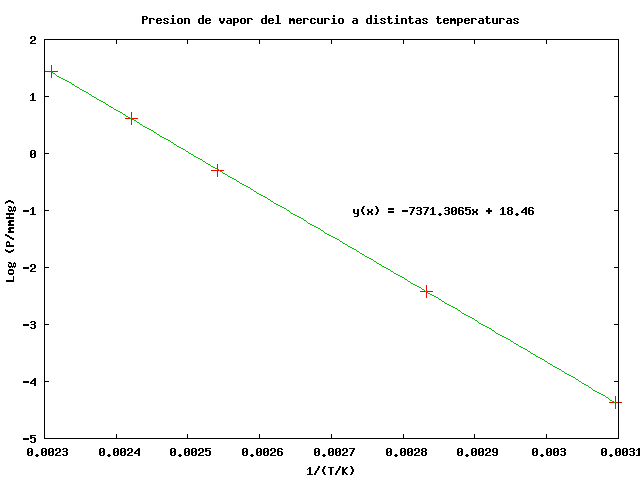
\includegraphics[scale=0.8]{figure8.png}
\end{center}


 \item \textbf{\textit{(McQuarrie 23-20)} Determinar el valor de $dT/dP$ para el agua en su punto de ebullici\'on normal de $373.15\;\mbox{K}$ dado que el valor de la entalp\'ia molar de vaporizaci\'on es $40.65\;\mbox{kJ}\cdot\mbox{mol}^{-1}$ y las densidades del l\'iquido y el vapor son $0.9584\;\mbox{g}\cdot\mbox{mL}^{-1}$ y $0.6010\;\mbox{g}\cdot\mbox{L}^{-1}$, respectivamente. Estimar el punto de ebullici\'on del agua a $2\;\mbox{atm}$.} % Problema 9-20

% Agregar.

 \item \textbf{\textit{(Chang 6.26)} El punto normal de ebullici\'on del etanol es de $78.3\celsius$ y su entalp\'ia molar de vaporizaci\'on es de $39.3\;\mbox{kJ}\cdot\mbox{mol}^{-1}$. ?`Cu\'al es su presi\'on de vapor a $30\celsius$?} % Problema 6.26 de Chang

% Agregar.

\end{enumerate}

\end{document}
